\documentclass[aps,twocolumn,secnumarabic,nobalancelastpage,amsmath,amssymb,
nofootinbib,superscriptaddress]{revtex4-1}


\usepackage{graphics}       % standard graphics specifications
\usepackage{graphicx}       % alternative graphics specifications
\usepackage{longtable}      % helps with long table options
\usepackage{url}            % for on-line citations
\usepackage{bm}             % special 'bold-math' package
\usepackage[ngerman]{babel} % deutsche Siblentrennung
\usepackage[utf8]{inputenc} % Umlaute
\usepackage{upgreek}        % aufrechte (nicht-kursive) griech. Buchstaben

\def\andname{\hspace*{-0.5em},} % definiert die Trennung zwischen 2 Autoren neu

% Titelseite
\begin{document}
\title{Compton-Effekt}
\author         {Ch. Egerland}
\email[Email: ]{egerlanc@physik.hu-berlin.de}
\author         {M. Pfeifer}

\email[Email: ]{max.pfeifer@physik.hu-berlin.de}
\affiliation    {Humboldt-Universität zu Berlin, Institut für Physik}
\date[Versuchsdatum: ]{13.06.2017}

%%%%%%%%%%%%%%%%%%%%%%%%%%%%%%%%%%%%%%%%%%%%%%%%%%%%%%%%%%%%%%%%%%%%%%%%%%%%%%%%
\begin{abstract}
  \noindent Gegenstand des Versuches ist die Untersuchung der Compton-Streuung von \textsuperscript{137}Cs-Photonen an einem Aluminium-Streutarget.
  Dazu werden die Spektren von drei Gammastrahlern (\textsuperscript{133}Ba, \textsuperscript{22}Na, \textsuperscript{137}Cs), sowie das Hintergrundrauschen
  mithilfe eines Szintillator-basierten Messsystems aufgenommen. Damit werden Aussagen über das Auflösungsvermögen der Apparatur und den qualitativen Verlauf der
  Spektren getroffen und schließlich der totale Wirkungsquerschnitt für \textsuperscript{137}Cs mit Korrekturen berechnet.
\end{abstract}


\maketitle


%%%%%%%%%%%%%%%%%%%%%%%%%%%%%%%%%%%%%%%%%%%%%%%%%%%%%%%%%%%%%%%%%%%%%%%%%%%%%%%%

\section{Zur Theorie des Compton-Effektes}
Der Compton-Effekt ist ein Phänomen, welches bei der Streuung von Photonen an
Teilchen beobachtet wird. Hierbei gibt das Photon einen Teil seiner Energie an das
ruhende Teilchen ab, wodurch die Wellenlänge des Photons steigt und das Teilchen
sich bewegt. Dieser Mechanismus ist in Abbildung~\ref{fig:kinematik} veranschaulicht.
Die Energie des gestreuten $\gamma$-Quants ist gegeben durch:

  \begin{equation}
    E^* = \frac{E_0}{1+\gamma(1- cos \theta)}
    \label{eq:streuenergie}
  \end{equation}

Hierbei ist $\theta$ der Streuwinkel und $\gamma = E_0/mc^2$ das Verhältnis der
Energie des eintreffenden Photons zur Ruheenergie des Elektrons. Man sieht, dass
dieser Effekt sich erst für hohe Photonenergien (also $\gamma >> 1$) bemerkbar
macht.

\begin{figure}[h]
  \centering
  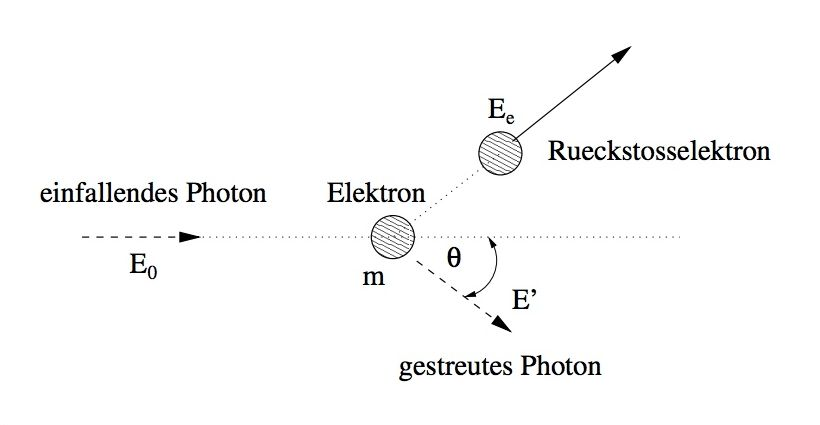
\includegraphics[width=0.5\textwidth]{comptstreu_schema.jpg}
  \caption{\label{fig:kinematik} Kinematik des Compton-Effekts aus \cite{skript07}.}
\end{figure}

Der korrekte differentielle Wirkungsquerschnitt, der die Winkelverteilung des
Compton-Effektes beschreibt, ist durch die Klein-Nishina-Formel gegeben:

  \begin{equation}
    \frac{d \sigma}{d \Omega} = \frac{r_0^2}{2} \left( \frac{E^*}{E_0} \right)^2
    \left( \frac{E_0}{E^*} + \frac{E^*}{E_0} - sin^2 \theta    \right)
    \label{eq:kleinnishina}
  \end{equation}

Aus dieser Formel folgt, dass es eine Vorwärts-Rückwärts-Asymmetrie gibt, d.h.
es werden mehr Photonen in die Vorwärtsrichtung, als in die Rückwärtsrichtung
gestreut.


%%%%%%%%%%%%%%%%%%%%%%%%%%%%%%%%%%%%%%%%%%%%%%%%%%%%%%%%%%%%%%%%%%%%%%%%%%%%%%%%
\section{Experiment}
Der Versuchsaufbau ist in Abbildung ~\ref{fig:aufbau} gezeigt. Die Photonen treten
aus der Strahlungsquelle (Daten in Tabelle ~\ref{tab:materialien}) in den Kolliminator
welcher dafür sorgt, dass die Photonen aus nahezu 0 Grad kommen. Das Aluminium-
Streutarget ist herausnehmbar.

\begin{figure}[h]
  \centering
  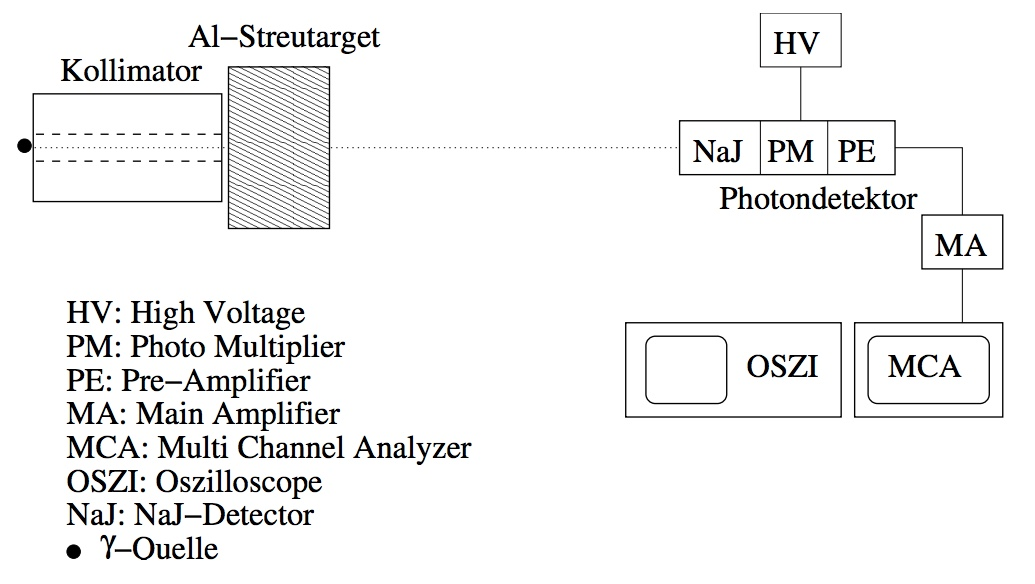
\includegraphics[width=0.5\textwidth]{aufbau.jpeg}
  \caption{\label{fig:aufbau} Versuchsaufbau aus \cite{skript07}.}
\end{figure}

Die Photonen treffen auf den Detektor, der in unserem
Fall aus einem mit Thallium dotierten NaJ-Szintillator besteht. Ein eintreffendes Photon
erzeugt im NaJ-Kristall ein Elektron-Loch-Paar welches sich zum Aktivatorzentrum
(Thallium) bewegt und dieses anregt. Durch Emission von Licht kehrt das Thallium
nun wieder in seinen Grundzustand zurück. Die aus dem Detektor gelösten Photonen
werden nun im Photomultiplier verstärkt. Hierbei trifft ein Photon auf den
Photomultiplier und löst durch den Photoeffekt ein Elektron, welches im weiteren
Verlauf weitere Elektronen aus den Dynoden herausschlägt (die sogenannten
Sekundärelektronen). Somit entsteht eine Spannung, welche wir als proportional zur
Energie der am Szintillator eintreffenden Photonen betrachten können. Diese
Spannung wird durch zwei OP Amplifier verstärkt und gelangt nun in den Multi Channel
Analyzer, welcher dafür sorgt, dass die eintreffenden Impulse mit verschiedener
Amplitude entsprechend diese einem Kanal zugeordnet werden. Diese Kanäle können
wir am PC auslesen und in einem Histogramm darstellen, wir sehen also ein Diagramm,
dass uns die Counts in den jeweiligen Kanälen zeigt. Daraus lässt sich mithilfe einer Kalibrationskurve,
die den Kanälen eine Energie zuordnet, das Energiespektrum bestimmen.

Zunächst ist es aus gesundheitlichen Erwägungen erforderlich, die Äquivalentdosis zu bestimmen, der man

\begin{table}[h]
\begin{ruledtabular}
\begin{tabular}{cccc}
 Präparat & $\gamma$-Energie in MeV & Aktivität (kBq) & Halbwertszeit\\
\hline
^{133} Ba & 0.356 & 397 & 10.54a \\
^{22} Na & 0.511 & 374 & 2.603a \\
^{137} Cs & 0.662 & 371 & 30.17a \\
\end{tabular}
\end{ruledtabular}
\caption{\label{tab:materialien} Daten der Photonenquellen ermittelt am 01.11.1996
mit einem Fehler von 4\%.}
\end{table}

\noindent während des Versuches ausgesetzt ist. Hierfür wird eine Experimentierdauer von 12 Stunden und eine
vollständige Absorption der Probenstrahlung angenommen. Die Äquivalentdosis H ist im Falle von Photonen
gleich der Dosis D \cite{qfaktor}. Die Dosisleistung ist definiert als

\begin{equation}
  \dot{D} = \frac{E_\gamma \cdot A}{m}
\end{equation}

\noindent mit der bestrahlten Masse $m$, der Aktivität $A$ der Photonenquelle und der Photonenenergie $E_\gamma$, wobei die Aktivität ein
zeitlich exponentiell abfallendes Verhalten zeigt:

\begin{equation}
  A(t)=A_0}\cdot exp\left( -\frac{t}{\tau}\right) =A_0\cdot exp\left(-\frac{t}{t_{1/2}}\cdot ln(2)\right)
\end{equation}

Dabei bezeichnet $A_0$ die Aktivität der Quelle am 01.11.1996 (s. Tabelle 1). Durch Integration der Dosisleistungen über die Zeit und Aufsummieren
der Dosisbeiträge der drei Proben gelangt man unter Annahme einer bestrahlten Masse von $m\approx 75$kg zu einer maximalen Äquivalentdosis von 17,5 $\upmu\text{Sv}$ (s. Anhang A1-A2).
Das entspricht einem Zuwachs der durchschnittlichen jährlichen Strahlungsbelastung ($\approx 2,1$ mSv \cite{jdosis}) um 0,8\%.

Da das Signal des Szintillators einen Vor- und Hauptverstärker durchläuft, ist die Messung einer Totzeit unterworfen. Das Messprogramm (MAESTRO)
quantifiziert diese Totzeit bereits und liefert Werte in der Größenordnung von 3 $\upmu\text{s}$ bis 17 $\upmu\text{s}$. Eine grafische, softwareunabhängige Abschätzung mit
dem Oszilloskop ergibt ähnliche Totzeiten in der Größenordnung von 8 $\upmu\text{s}$. Die Zeit, die der Detektor zur Messung eines Ereignisses benötigt, beträgt mit 6 ms drei
Größenordnungen mehr als die Totzeit, womit diese vernachlässigt werden kann. %HIER VLLT NOCH VGL WIE VIELE SIGNALE ABSOLUT VERLOREN GEGANGEN SIND



%%%%%%%%%%%%%%%%%%%%%%%%%%%%%%%%%%%%%%%%%%%%%%%%%%%%%%%%%%%%%%%%%%%%%%%%%%%%%%%%
\section{Daten und Analyse}

Lorem ipsum dolor sit amet, consectetur adipiscing elit. Nam id facilisis ligula,
a ultrices nibh. Nullam suscipit tellus nec mauris fermentum, ornare luctus neque
tincidunt. Aenean commodo tincidunt varius. Phasellus faucibus metus non erat
consectetur bibendum. Duis et luctus risus, at egestas justo. Nunc eleifend lacus
ac laoreet scelerisque. Aenean cursus dignissim magna in ultrices. In eget nisl
quis nisi. Tabelle \ref{tab:table1}:







%%%%%%%%%%%%%%%%%%%%%%%%%%%%%%%%%%%%%%%%%%%%%%%%%%%%%%%%%%%%%%%%%%%%%%%%%%%%%%%%
\section{Schlussfolgerung}

Schlussoflgerung, sollten wir mal was von nem Buch oder so entnehmen nutzen wir:


\begin{quote}
  Ein Zitat mit Referenz auf das Buch\cite{melissinos1966}
\end{quote}

Lorem ipsum dolor sit amet, consectetur adipiscing elit. Nam id facilisis ligula,
a ultrices nibh. Nullam suscipit tellus nec mauris fermentum, ornare luctus neque
tincidunt. Aenean commodo tincidunt varius. Phasellus faucibus metus non erat
consectetur bibendum. Duis et luctus risus, at egestas justo. Nunc eleifend lacus
ac laoreet scelerisque. Aenean cursus dignissim magna in ultrices. In eget nisl
quis nisi.


%%%%%%%%%%%%%%%%%%%%%%%%%%%%%%%%%%%%%%%%%%%%%%%%%%%%%%%%%%%%%%%%%%%%%%%%%%%%%%%%
\bibliography{sample-paper}
\bibliographystyle{prsty}
\begin{thebibliography}{99}
\bibitem{skript07}O.Epler, U. Schwanke, Compton-Effekt (Versuchsskript),  [2007]
\bibitem{qfaktor}H.Krieger, Grundlagen der Strahlungsphysik und des Strahlenschutzes (S. 323), Springer Verlag, 4. Auflage [2004]
\bibitem{jdosis}Bundesamt für Strahlenschutz, "Wie hoch ist die natürliche Strahlenbelastung in Deutschland?\grqq\: (unter http://www.bfs.de/DE/themen/ion/umwelt/natuerliche-strahlenbelastung/natuerliche-strahlenbelastung_node.html)
\end{thebibliography}


%%%%%%%%%%%%%%%%%%%%%%%%%%%%%%%%%%%%%%%%%%%%%%%%%%%%%%%%%%%%%%%%%%%%%%%%%%%%%%%%
\clearpage
\appendix

\section{Sonstiges}

% Strahlendosisberechnung
\begin{equation}
  D = \sum\limits_{i=1}^3 \int\limits_{t_1}^{t_2} \! \dot{D_i}(t) \, \mathrm{d}t = \frac{1}{m}\sum\limits_{i=1}^3
  \frac{1}{E_{\gamma,i}} \int\limits_{t_1}^{t_2} \! A_{i}(t) \, \mathrm{d}t  \newline
\end{equation}
mit $t_1 = 20,263a$ und $t_2 = 20,263a$ + 12h
\begin{equation}
  \begin{gathered}
    D_i = \cfrac{E_{\gamma,i}}{m} \int\limits_{t_1}^{t_2} \! A_i(t) \, \mathrm{d}t \\
    = \cfrac{E_{\gamma,i}\cdot A_{0,i}}{m} \int\limits_{t_1}^{t_2} \! exp\left(-\frac{t}{t_{1/2}}\cdot ln(2)\right) \, \mathrm{d}t
  \end{gathered}
\end{equation}
\Rightarrow D_{Ba} = 3.36\:$\upmu\text{Sv}$,\: D_{Na} = 0.07\:$\upmu\text{Sv}$,\: D_{Cs} = 14.11\:$\upmu\text{Sv}$
\vspace{3em}

\begin{figure}[h]
  \centering
  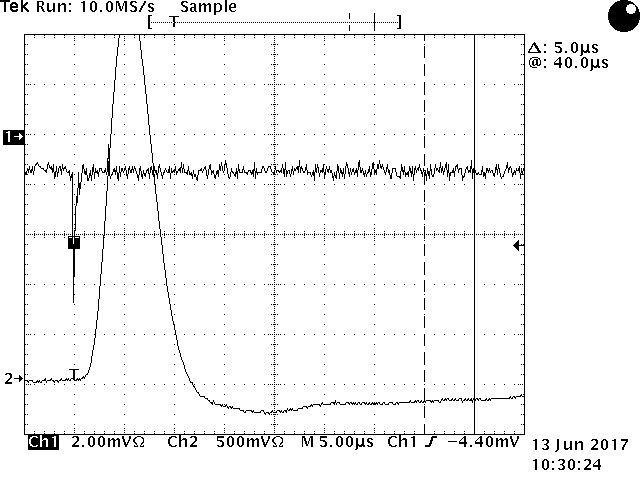
\includegraphics[width=0.5\textwidth]{../Messung/OsziVerstaerkerkurve/TEK00009.jpg}
  \caption{\label{fig:aufbau} Vor- und Hauptverstärkersignal Oszilloskop}
\end{figure}

Hier sehen wir einen Beispiel Anhang und so könnte man Code in Latex einbinden:
\begin{verbatim}
> mkdir ~/8.13
> mkdir ~/8.13/papers
> mkdir ~/8.13/papers/template
> cd ~/8.13/papers/template
\end{verbatim}


%%%%%%%%%%%%%%%%%%%%%%%%%%%%%%%%%%%%%%%%%%%%%%%%%%%%%%%%%%%%%%%%%%%%%%%%%%%%%%%%


\end{document}
